\section{Auswertung}
\label{sec:Auswertung}
Die in \autoref{sec:Auswertung} gezeigten Grafiken und Rechnungen sind mithilfe der Python-Bibliotheken Matplotlib \cite{matplotlib}, Scipy \cite{scipy} und Numpy \cite{numpy}
erstellt worden.

\subsection{Charakteristik des Geiger-Müller Zählrohres}
Die aus dem ersten Teil der Durchführung aufgenommenen Messwerte sind in \autoref{tab:1} dargesellt.

\begin{table}[H]
  \centering
  \caption{Impulse $N$, Spannung $U$ und Strom $I$ aus der ersten Messreihe.}
  \begin{tabular}{c c c}
      \toprule
      {$N[\unit{\frac{Imp}{60s}}]$} & {$U[\unit{V}]$} & {$I[\unit{\micro A}]$}\\
      \midrule
      10557 & 320 & 0.1\\
      13259 & 330 & 0.2\\
      13297 & 340 & 0.2\\
      13426 & 350 & 0.2\\
      13276 & 360 & 0.2\\
      13468 & 370 & 0.2\\
      13563 & 380 & 0.2\\
      13396 & 390 & 0.2\\
      13520 & 400 & 0.2\\
      13489 & 410 & 0.3\\
      13616 & 420 & 0.3\\
      13774 & 430 & 0.3\\
      13775 & 450 & 0.3\\
      13740 & 460 & 0.4\\
      13747 & 470 & 0.4\\
      13668 & 480 & 0.4\\
      14129 & 490 & 0.4\\
      13755 & 500 & 0.4\\
      13735 & 510 & 0.4\\
      13610 & 520 & 0.5\\
      13551 & 530 & 0.5\\
      13783 & 540 & 0.5\\
      13660 & 550 & 0.5\\
      13681 & 570 & 0.6\\
      13950 & 590 & 0.6\\
      14046 & 610 & 0.7\\
      13950 & 630 & 0.7\\
      14112 & 650 & 0.8\\
      14335 & 670 & 0.8\\
      14271 & 690 & 0.8\\
      14821 & 710 & 0.8\\
      15229 & 730 & 0.9\\
      15896 & 750 & 1.0\\
      \bottomrule
  \end{tabular}
  \label{tab:1}
\end{table}

Nach \autoref{sec:Messunsicherheit} ergibt sich der absolute Fehler mit $\sqrt{N}$.

Um eine Aussage über die Güte des benutzten Zählrohrs tätigen zu können, werden die Impulse pro 60s $N$ gegen die
Betriebsspannung $U$ aufgetragen. Somit entsteht \autoref{fig:kennlinie}.
Mit einer linearen Ausgleichsrechnung kann eine Gerade durch die Kennlinie des Zählrohrs gelegt werden.
Mit der Funktion linregress aus der SciPy Bibliothek \cite{scipy} ergeben sich folgende Parameter für die Gerade der Form $aU + b$:
\begin{align*}
  a &= \SI{2.26(0.29)}{\frac{1}{V}}\\
  \text{und } b &= 12617 \pm 150.
\end{align*}

\begin{figure}[H]
  \includegraphics[width=\textwidth]{build/kennlinie.pdf}
  \caption{Plot der Ergebnisse aus \autoref{tab:1} mit Fehler und Ausgleichsgerade.}
  \label{fig:kennlinie}
\end{figure}

Daraus kann der Arbeitspunkt $U_A$ des Zählrohrs bei $\approx \SI{420}{V}$ und die Plateaulänge zu $L = 360$ abgelesen werden.
Der prozentuale Plateauanstieg ergibt $s_{\%} = 7\%$.

\subsection{Bestimmung der freigesetzten Ladung}
Aus den aufgenommenen Messwerten kann mit \autoref{eq:Z} die freigesetzte Ladung pro detektiertem Teilchen berechnet werden.
Die Ergebnisse sind in \autoref{tab:2} aufgelistet.

\begin{table}[H]
  \centering
  \caption{Impulse $N$, Spannung $U$ und Strom $I$ aus der ersten Messreihe.}
  \begin{tabular}{c c c}
      \toprule
      {$N[\unit{\frac{Imp}{60s}}]$} & {$Z \cdot 10^6$} & {$I[\unit{\micro A}]$}\\
      \midrule
      10557$\pm$102 & 59.1$\pm$0.5 & 0.1\\
      13259$\pm$115 & 94.1$\pm$0.8 & 0.2\\
      13775$\pm$117 & 135.9$\pm$1.1 & 0.3\\
      13735$\pm$117 & 181.7$\pm$1.5 & 0.4\\
      13660$\pm$116 & 229.3$\pm$1.9 & 0.5\\
      13681$\pm$118 & 268.4$\pm$2.2 & 0.6\\
      14046$\pm$118 & 311.0$\pm$2.6 & 0.7\\
      14821$\pm$121 & 336.9$\pm$2.7 & 0.8\\
      15229$\pm$123 & 368.8$\pm$2.9 & 0.9\\
      15896$\pm$126 & 392.6$\pm$3.1 & 1.0\\
      \bottomrule
  \end{tabular}
  \label{tab:2}
\end{table}

Wird die Anzahl der Ladungsträger als Funktion der Betriebsspannung aufgetragen entsteht \autoref{fig:2}.

\begin{figure}[H]
  \includegraphics[width=\textwidth]{build/strom.pdf}
  \caption{Plot der Ergebnisse aus \autoref{tab:2} mit Fehler.}
  \label{fig:2}
\end{figure}

\subsection{Bestimmung der Totzeit}
Die Messung mit der Zwei-Quellen-Methode ergab folgende Messwerte:
\begin{align*}
  N_1 &= \SI{9.386(0.031)e+04}{\frac{\text{Imp}}{120s}}\\
  N_2 &= \SI{1.470(0.004)e+05}{\frac{\text{Imp}}{120s}}\\
  \text{und } N_{1+2} &= \SI{2.238(0.005)e+05}{\frac{\text{Imp}}{120s}}\\.
\end{align*}

Daraus lässt sich nach \autoref{eq:totzeit} die Totzeit berechnen:
\begin{equation*}
  \tau_1 = \SI{104(5)}{\micro\s}.
\end{equation*}
Ebenfalls kann die Totzeit mithilfe eines Oszilloskops abgeschätzt werden. Wenn die Internsität der Strahlungsquelle hoch genug ist,
kann durch die Zeitdifferent zweier Impulse die Totzeit abgelesen werden.
\\
\\
Wendet man diese Methode auf \autoref{fig:totzeit} an, so lässt sich die Totzeit zu $\tau_2 = \SI{125(5)}{\micro\s}$ ablesen.
\begin{figure}[H]
  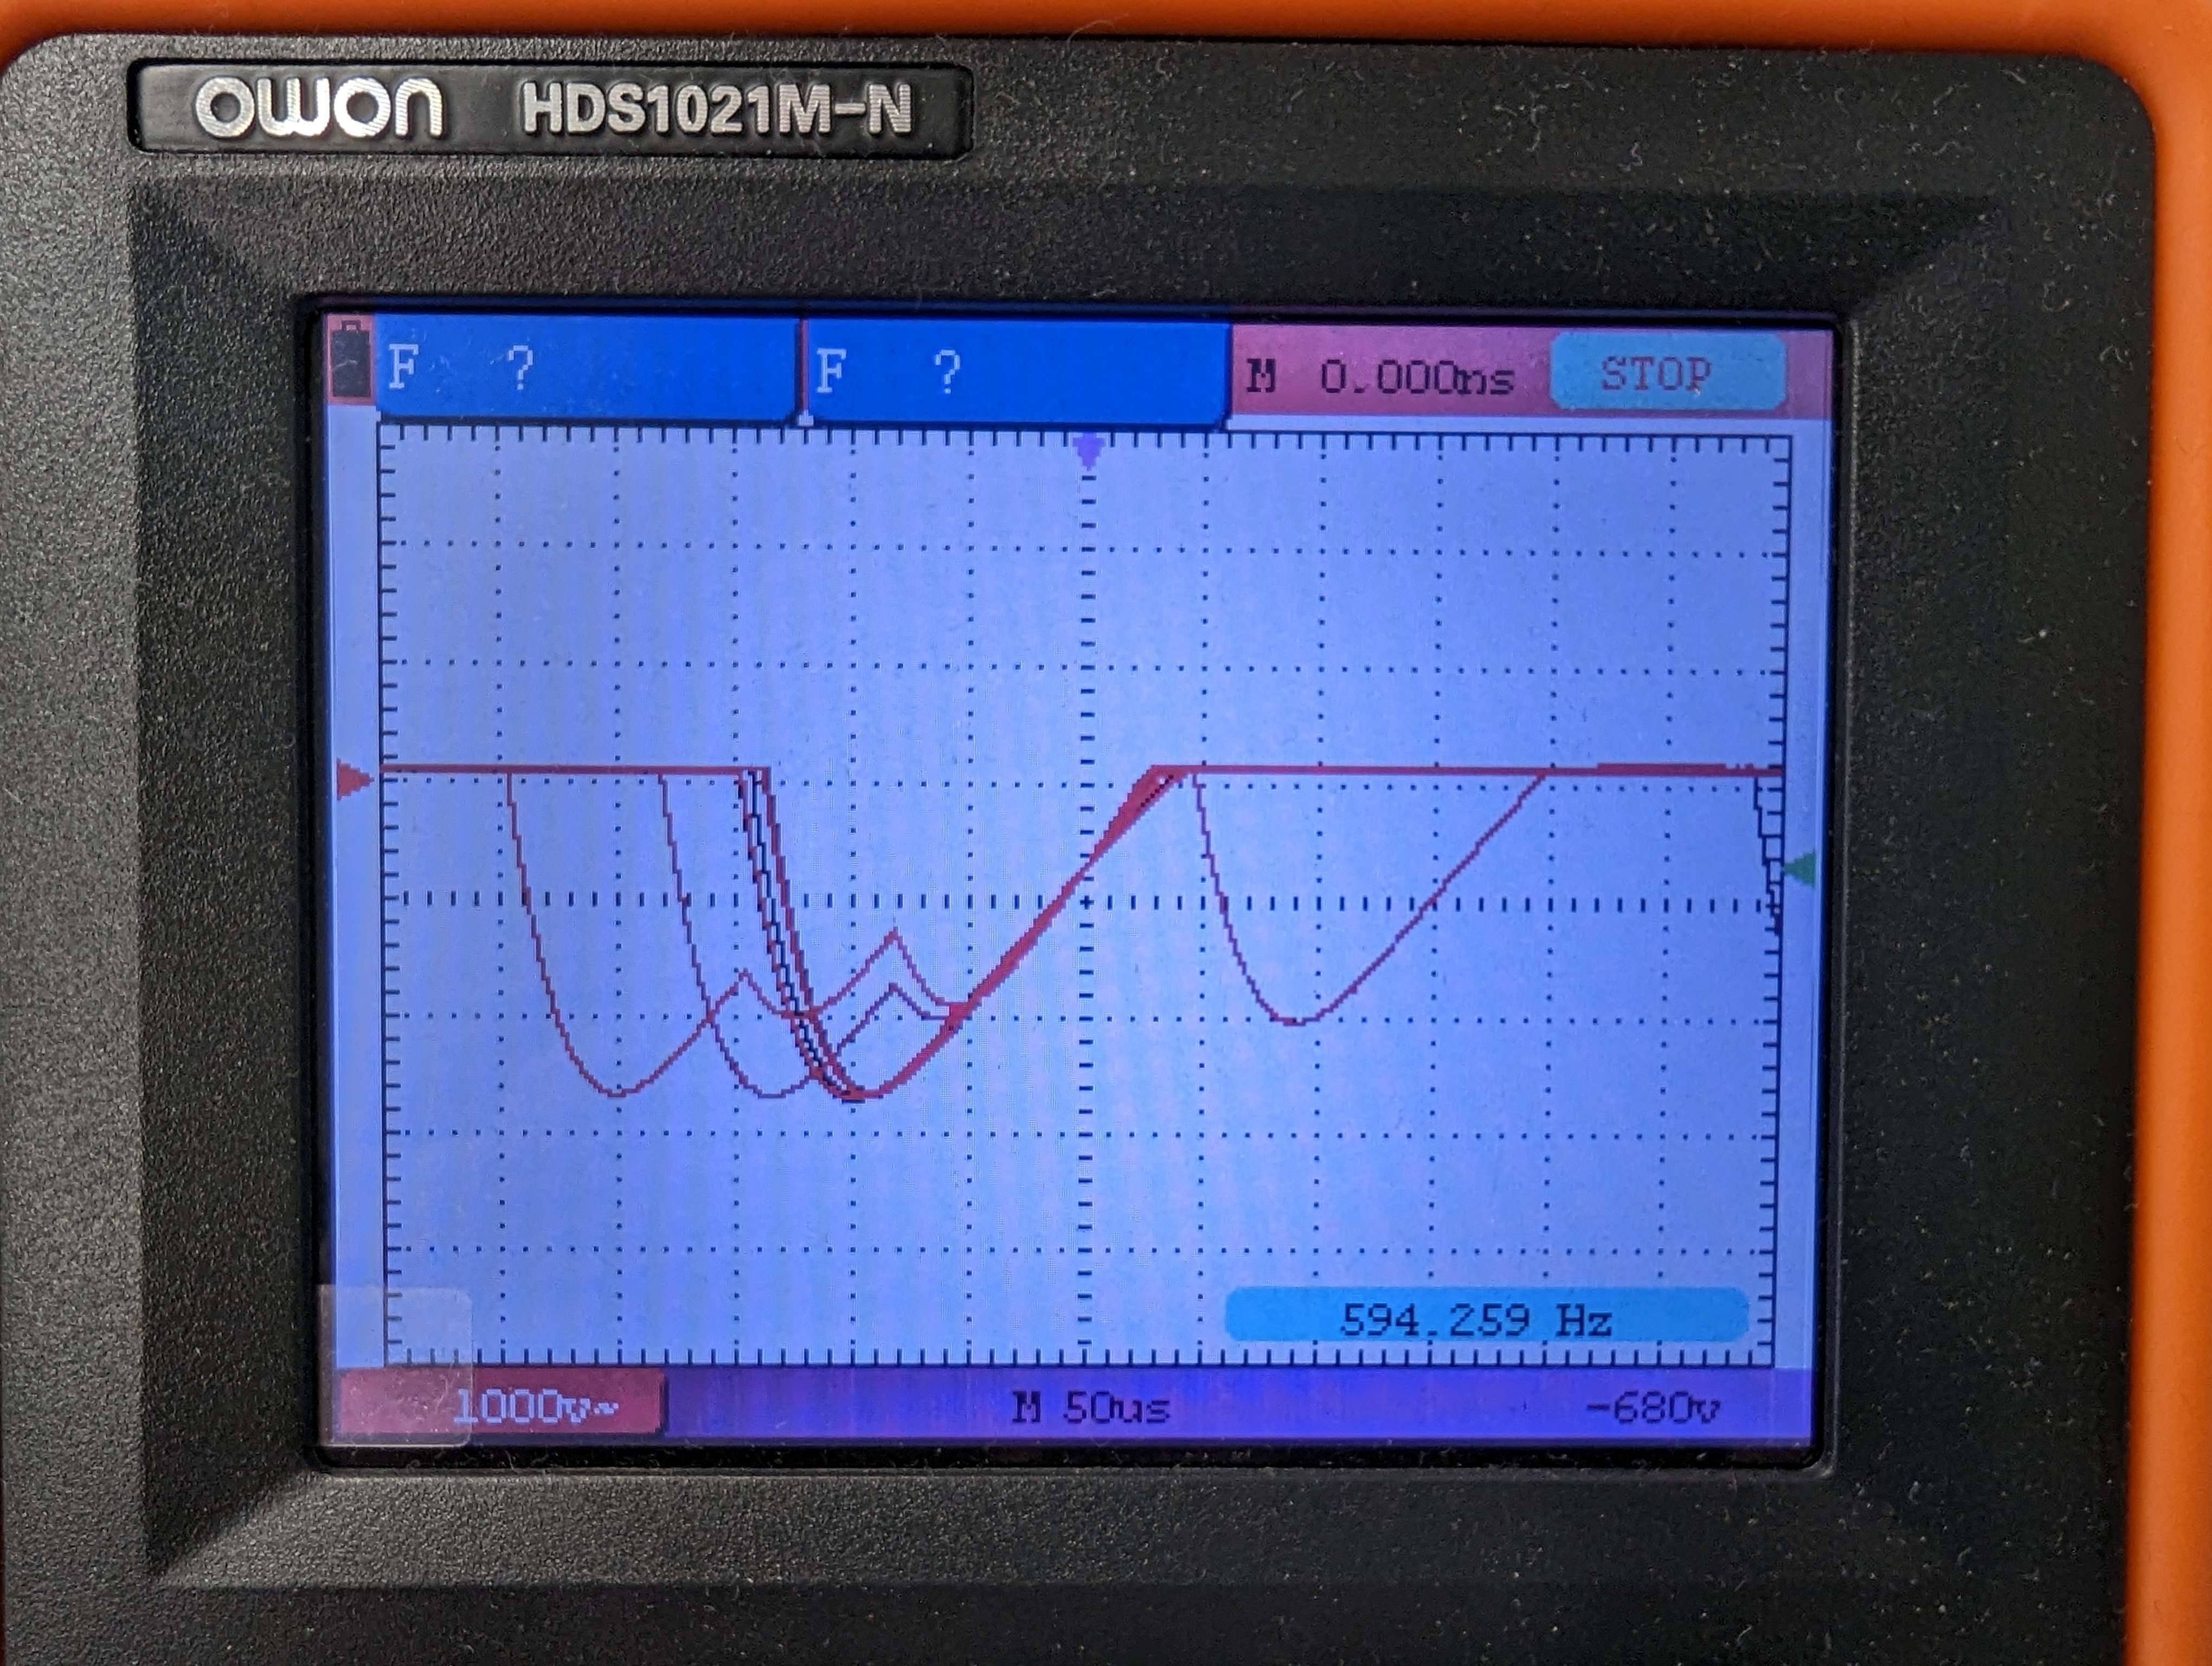
\includegraphics[width=\textwidth]{content/oszilloskop.jpg}
  \caption{Bild des Oszilloskops zur Abschätzung der Totzeit.}
  \label{fig:totzeit}
\end{figure}

\newpage